\chapter{Tests}

\section{Schematics}

float barrier command to ensure that text stays close to the picture but no text from after the pciture.

\subsection{part 1}

\begin{figure}[ht]
    \centering
    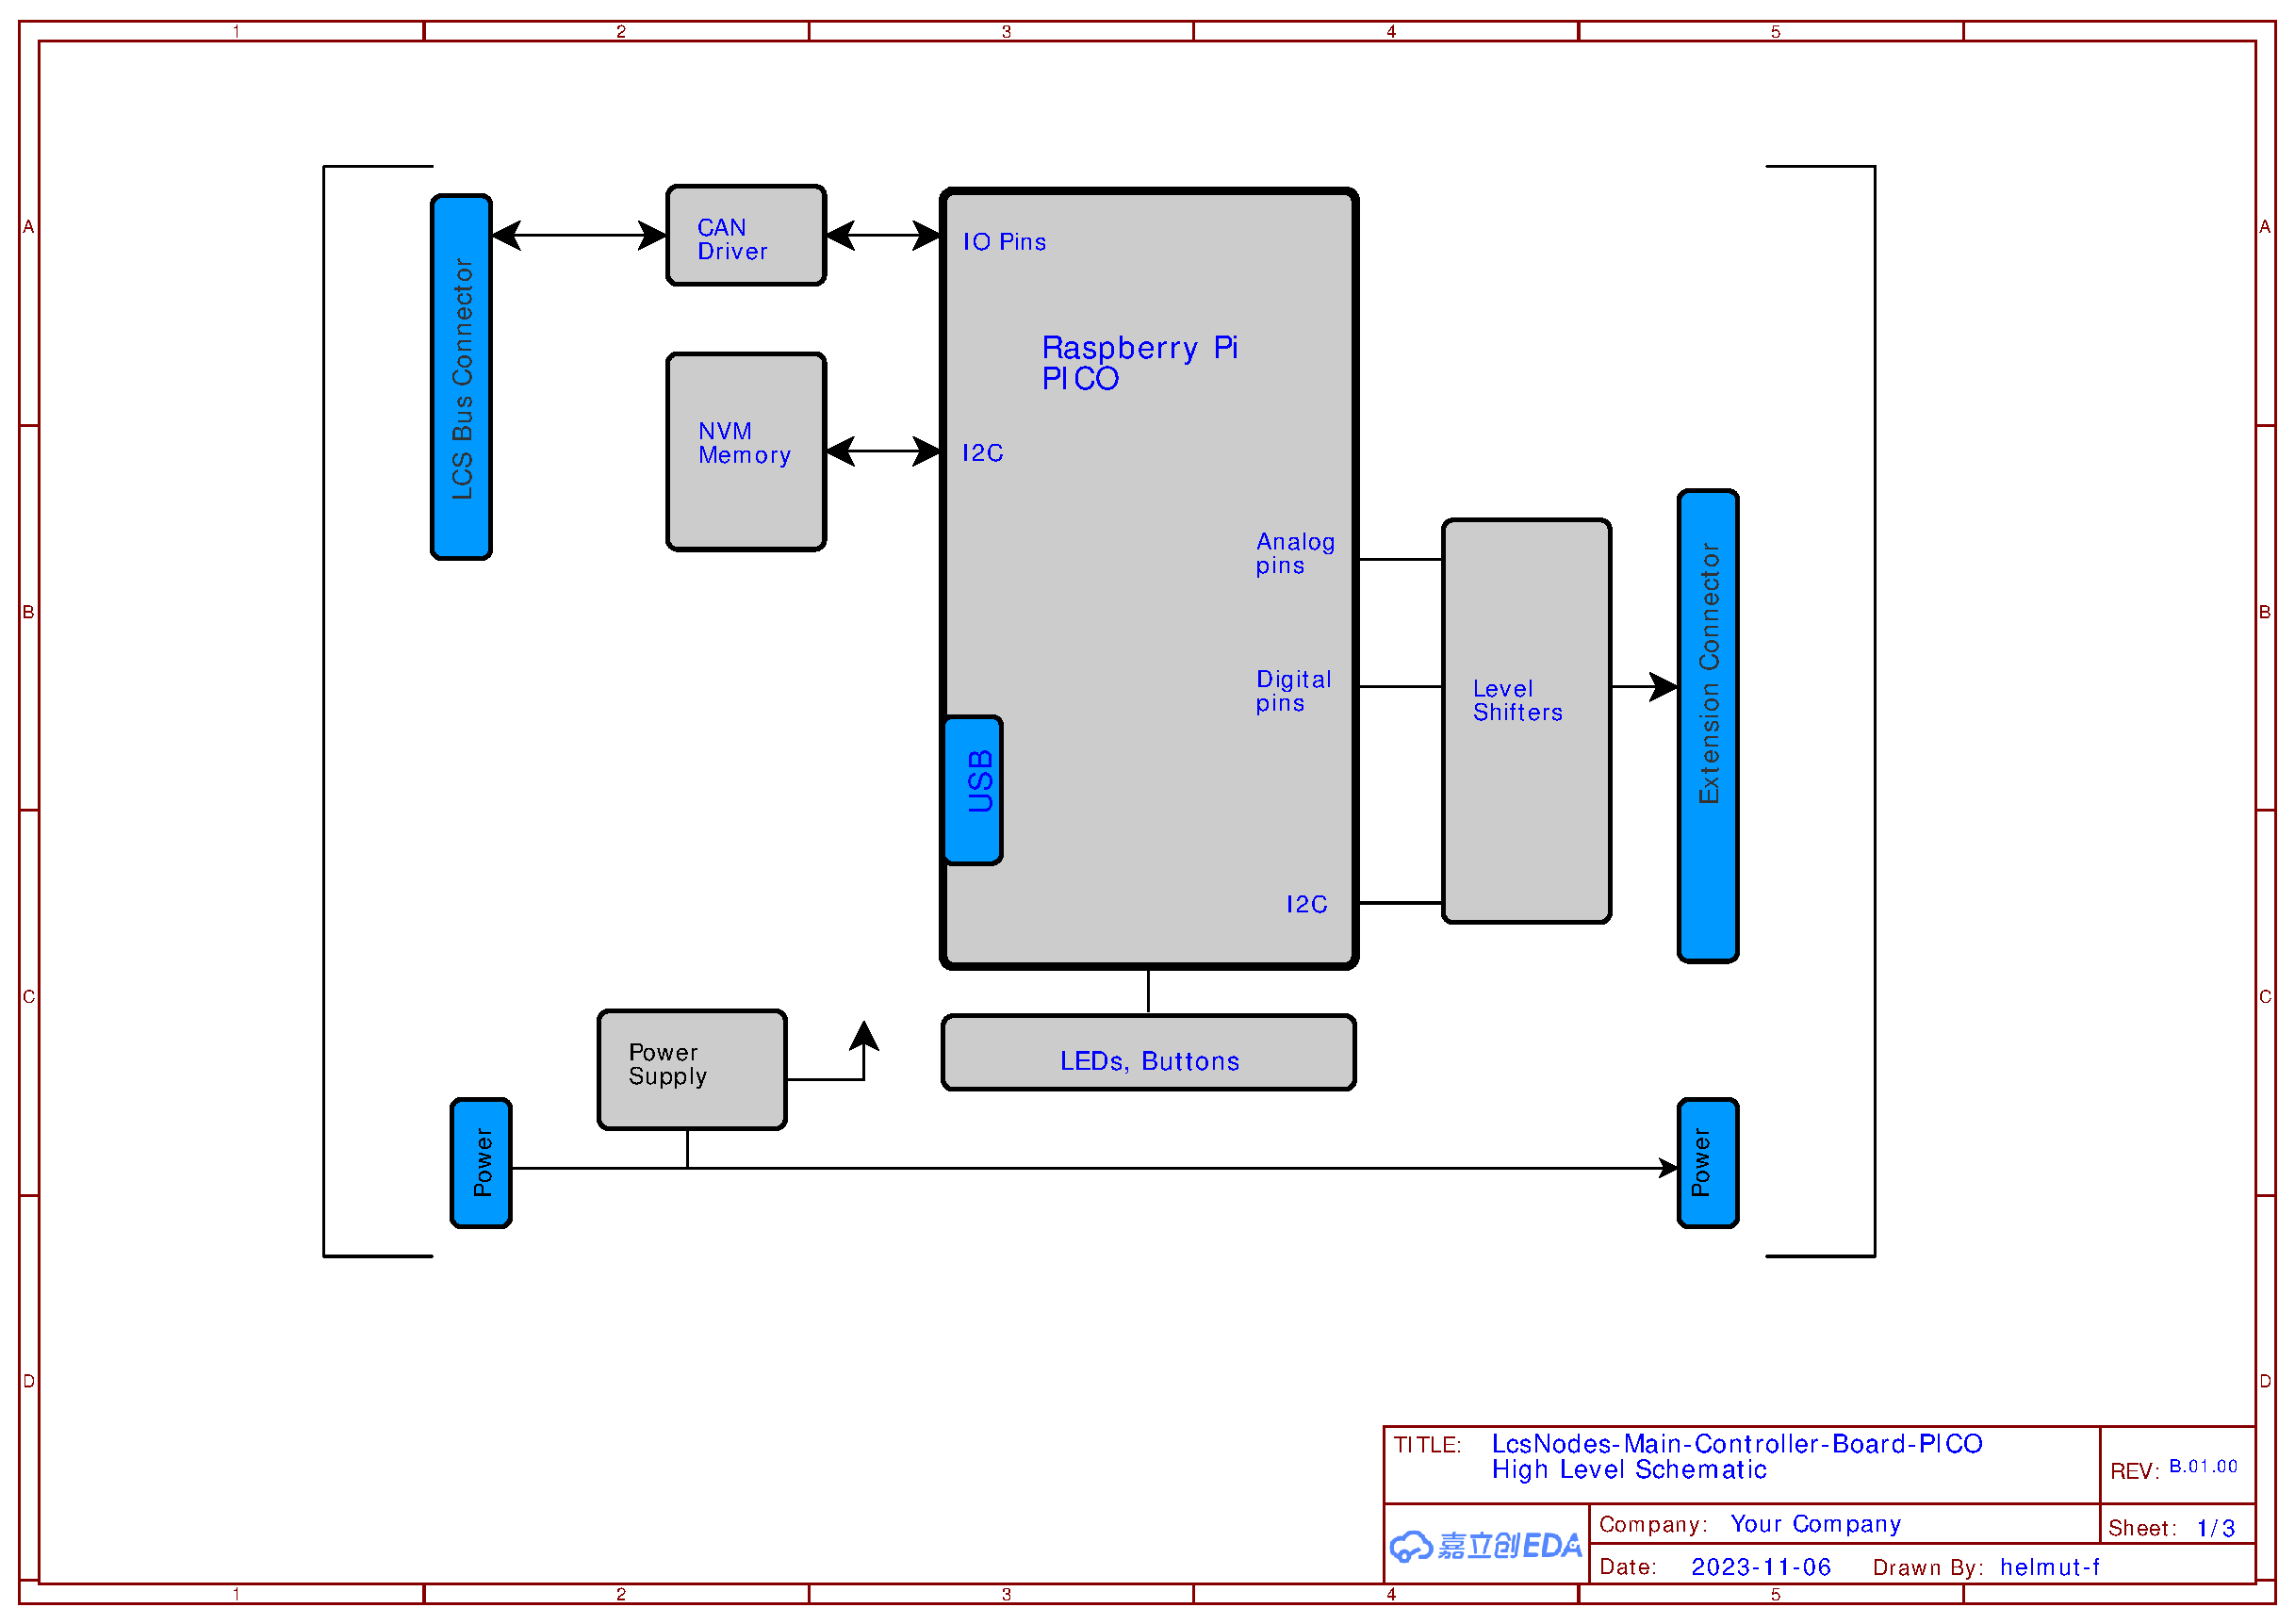
\includegraphics[page=1, width=\textwidth]{./schematics/Schematic_LcsNodes-Main-Controller-Board-B.01.00.pdf}
\end{figure}

\FloatBarrier

\subsection{part 2}
\begin{figure}[ht]
    \centering
    \includegraphics[page=2, width=\textwidth]{./schematics/Schematic_LcsNodes-Main-Controller-Board-B.01.00.pdf}
\end{figure}

\FloatBarrier

\subsection{part 3}
\begin{figure}[ht]
    \centering
    \includegraphics[page=3, width=\textwidth]{./schematics/Schematic_LcsNodes-Main-Controller-Board-B.01.00.pdf}
\end{figure}

\FloatBarrier


\section{Code Snippets}

\lstset{style=listingstyle}
\begin{lstlisting}

    int main( int argc, char **argv ) {

        return( 0 );
    }
    
\end{lstlisting}


\section{Lists}

\subsection{ a simple list}

\begin{itemize}
    \item First bullet point
    \item Second bullet point
    \item Third bullet point
\end{itemize}


